\section{PS3a: N-Body Simulation (Static)}\label{sec:ps3a}
\graphicspath{{ps3a}}
\subsection{Discussion:}\label{sec:ps3a:disc}
We have been through our school education where we learned about solar systems. We wondered how these planets are implemented as an animation to display on the screen. Well to answer these thoughts, such assignments are created to know how to create animation. At the first part we will create a static animation of the solar system and in the second part we will simulate the static bodies by using physics.


    The \textbf{PS3a} asks us to load and display static images of the planets.
    We are using two classes Universe and CelestialBody classes. The class CelestialBody is used to show any planet rendered in the universe, example: Our planet Earth. Universe class has a vector of CelestialBody and has a function to create the entire universe by accessing the vector.
    
    \textbf{We use the provided planets.txt file for this assignment: The values are as follows: } \newline
    \textbf{Inputs: 5 \newline Radius: 2.50e+11 }
    \begin{center}
 \begin{tabular}{||c c c c c c||} 
 \hline
 x-axis & y-axis & velocity of x-axis & velocity of y-axis & Mass & filename \\ [0.5ex] 
 \hline\hline
 1.4960e+1 & 0.0000e+00 & 0.0000e+00 & 2.9800e+04 & 5.9740e+24 &  earth.gif  \\ 
 \hline
 2.2790e+11 & 0.0000e+00 & 0.0000e+00 & 2.4100e+04 & 6.4190e+2 &  mars.gif  \\ 
 \hline
 5.7900e+10 & 0.0000e+00 & 0.0000e+00 &  4.7900e+04 &  3.3020e+23 &  mercury.gif  \\ 
 \hline
0.0000e+00 & 0.0000e+00 & 0.0000e+00 & 0.0000e+00 & 1.9890e+30 &  sun.gif  \\ 
 \hline
1.0820e+11  & 0.0000e+00 & 0.0000e+00 & 3.5000e+04 & 4.8690e+24 &  venus.gif  \\  
 \hline
\end{tabular}
\end{center}



\subsection{Key algorithms, Data structures and OO Designs used in this Assignment:}\label{sec:ps3a:kdo}
I used istream to read the data from planets.txt and ostream as output.Displays the planets in an SFML window.
       Reads input of file using < operator.  
       I did not use any smart pointers. Just used General Pointers.
       Simply added (space) key to exit from the window.
       used Address-operator for managing the addresses of variables and also the objects.
       I have not used any smart pointers. \newline
       \textbf{\colorbox{lime}{istream code:}}
       \begin{lstlisting}
       std::istream& operator>> (std::istream &data, CelestialBody &body) {

data >> body.x >> body.y >> body.vx >> body.vy >> body.mass >> body.filename;

if (!body.image.loadFromFile(body.filename))
    return data;
body.calculatePosition();
body.texture.loadFromImage(body.image);
body.sprite.setTexture(body.texture);
body.sprite.setPosition(body.rx, body.ry);
return data;

}
       \end{lstlisting}
              \textbf{\colorbox{lime}{ostream code:}}
       \begin{lstlisting}
       std::ostream& operator<< (std::ostream &outstream, CelestialBody &body){
outstream << "CelestialBody :  x:" << body.x << " y:";
outstream << body.y << " velx:" << body.vx << " vely:";
outstream << body.vy << " mass:" << body.mass << "";
outstream << " ~~x:" << body.rx << "  --- " << body.ry << "~~" << " " << body.filename << std::endl;
return outstream;
       \end{lstlisting}

\subsection{Images used:}\label{sec:ps3a:img}
\begin{figure}[h]
    \centering
    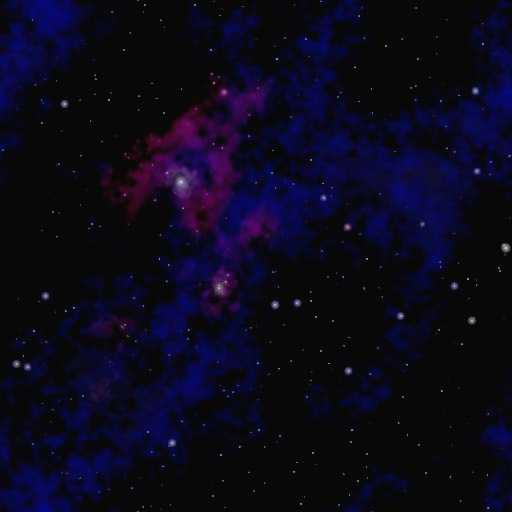
\includegraphics[width=0.5\textwidth]{ps3a/starfield.jpg}
    \caption{Background Image}
    \label{fig:ps3abg}
\end{figure}
\begin{figure}[h]
    \centering
    
\includegraphics[width=0.2\textwidth]{ps3a/earth.png}
    \caption{Background Image}
    \label{fig:earth}
\end{figure}
\begin{figure}[h]
    \centering
    
\includegraphics[width=0.2\textwidth]{ps3a/mars.png}
    \caption{Background Image}
    \label{fig:mars}
\end{figure}
\newpage
\begin{figure}[h]
    \centering
    
\includegraphics[width=0.2\textwidth]{ps3a/venus.png}
    \caption{Background Image}
    \label{fig:venus}
\end{figure}\begin{figure}[h]
    \centering
    
\includegraphics[width=0.2\textwidth]{ps3a/sun.png}
    \caption{Background Image}
    \label{fig:sun}
\end{figure}
\begin{figure}[h]
    \centering
    
\includegraphics[width=0.2\textwidth]{ps3a/mercury.png}
    \caption{Background Image}
    \label{fig:mercury}
\end{figure}
\newpage
\subsection{What I accomplished :}\label{sec:ps3a:accomplish}

I accomplished creating a solar system by the given input data. I created my first animated solar system. I am amazed that how physics can be implemented in the code.

\subsection{What I already knew :}\label{sec:ps3a:knew}

I knew how to add the background and use of the draw. I also knew how to take input from the file and display.
I knew how to create header files and implement them into the cpp files.


\subsection{What I learned :}\label{sec:ps3a:learn}

I learnt how to use physics in creating the solar model. I understood much use of the istream and ostream in this assignment. I understood the calculations required for the placement of the CelestialBodies.
         I was able to learn how to use unitary methods and also vectors in a good level.
         Honestly, I was weak in operator overloading but by doing this project I am able to grip on it.

\subsection{Challenges :}\label{sec:ps3a:challenges}
        I was unable to use smart pointers and few algorithm classes, so I kind of felt a difficulty in that.

\subsection{Acknowledgments :}\label{sec:ps3a:ack}
\textbf{Links :}
\begin{itemize}
    \item \url{https://www.sfml-dev.org/tutorials/2.5/graphics-sprite.php}
    \item \url{https://icarus.cs.weber.edu/~dab/cs1410/textbook/11.Operators/io_overload.html}
    \item \url{https://www.cplusplus.com/reference/vector/vector/}
    \item \url{https://www.sfml-dev.org/documentation/2.5.1/classsf_1_1Drawable.php}
    \item \url{https://stackoverflow.com/questions/34458791/making-custom-types-drawable-with-sfml}
\end{itemize}
\newpage


\subsection{Codebase}\label{sec:ps3a:code}

\textbf{\colorbox{pink}{Makefile}} \newline \textbf{This Makefile has no Linting as the program does not have any lints.}
\lstinputlisting[language=Make]{ps3a/Makefile}

\textbf{\colorbox{pink}{main.cpp}} \newline \textbf{The main file is important as it is base for creating a window and displaying the CelestialBodies on it.}
\lstinputlisting{ps3a/main.cpp}

\textbf{\colorbox{pink}{CelestialBody.hpp}} \newline \textbf{The CelestialBody.hpp contains the initializations of istream,ostream and variable and methods for the creation of the Nbodies.}
\lstinputlisting{ps3a/CelestialBody.hpp}

\newpage
\textbf{\colorbox{pink}{CelestialBody.cpp}} \newline \textbf{This is the file where the Celestial body data are taken by the istream and provide an accurate calculation for the position of them as well as provide the data of each CelestialBody on the terminal.}
\lstinputlisting{ps3a/CelestialBody.cpp}

\textbf{\colorbox{pink}{Universe.hpp}} \newline \textbf{This header file contains the declarations of few important variables such as numberOFplanets,radius and also methods.}
\lstinputlisting{ps3a/Universe.hpp}


\textbf{\colorbox{pink}{Universe.cpp}} \newline \textbf{This file sets radius and adds Body to window}
\lstinputlisting{ps3a/Universe.cpp}


\newpage
\subsection{Output:}\label{sec:ps3a:output}
\begin{figure}[h]
    \centering
    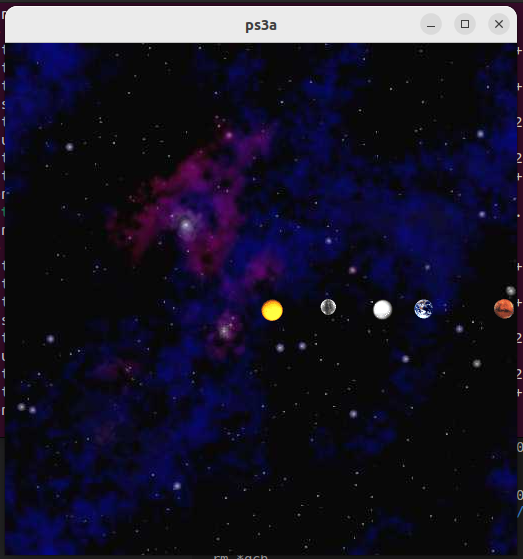
\includegraphics[width=1\textwidth]{ps3a/screenshot.png}
    \caption{NBody Simulation (static)}
    \label{fig:ps3a}
\end{figure}

\newpage
